\def\mytitle{IDE ASSIGNMENT}
\def\myauthor{TANGALLAMUDI RAMA SAI}
\def\contact{ramsaitangallamudi19@gmail.com}
\def\mymodule{Future Wireless Communications (FWC)}
\documentclass[journal,14pt,onecolumn]{IEEEtran}

\usepackage{setspace}
\usepackage{gensymb}
\usepackage{xcolor}
\usepackage{caption}
\usepackage[hyphens,spaces,obeyspaces]{url}
\usepackage[cmex10]{amsmath}
\usepackage{mathtools}
\singlespacing
\usepackage{amsthm}
\usepackage{mathrsfs}
\usepackage{txfonts}
\usepackage{stfloats}
\usepackage{cite}
\usepackage{cases}
\usepackage{subfig}
\usepackage{attachfile}
\usepackage{longtable}
\usepackage{multirow}
\twocolumn


\usepackage{graphicx}
\graphicspath{{./images/}}
\usepackage[colorlinks,linkcolor={black},citecolor={blue!80!black},urlcolor={blue!80!black}]{hyperref}
\usepackage[parfill]{parskip}
\usepackage{lmodern}
\usepackage{tikz}
\usepackage{circuitikz}
\usepackage{karnaugh-map}
\usepackage{pgf}
\usepackage[hyphenbreaks]{breakurl}

\usepackage{tabularx}
\usetikzlibrary{calc}

\renewcommand*\familydefault{\sfdefault}
\usepackage{watermark}
\usepackage{lipsum}
\usepackage{xcolor}
\usepackage{listings}
\usepackage{float}
\usepackage{titlesec}
\usepackage{enumitem}
\DeclareMathOperator*{\Res}{Res}
\renewcommand\thesection{\arabic{section}}
\renewcommand\thesubsection{\thesection.\arabic{subsection}}
\renewcommand\thesubsubsection{\thesubsection.\arabic{subsubsection}}

\renewcommand\thesectiondis{\arabic{section}}
\renewcommand\thesubsectiondis{\thesectiondis.\arabic{subsection}}
\renewcommand\thesubsubsectiondis{\thesubsectiondis.\arabic{subsubsection}}
\titlespacing{\subsection}{1pt}{\parskip}{3pt}
\titlespacing{\subsubsection}{0pt}{\parskip}{-\parskip}
\titlespacing{\paragraph}{0pt}{\parskip}{\parskip}
\newcommand{\figuremacro}[5]{
    \begin{figure}[#1]
        \centering
        \includegraphics[width=#5\columnwidth]{#2}
        \caption[#3]{\textbf{#3}#4}
        \label{fig:#2}
    \end{figure}
}

\lstset{
frame=single, 
breaklines=true,
columns=fullflexible
}
\title{\mytitle}
\author{\myauthor\hspace{1em}\\\contact\\IITH\hspace{0.5em}-\hspace{0.6em}\mymodule}
\date{20-12-2022}
\def\inputGnumericTable{}                                 %%
\lstset{
frame=single, 
breaklines =true,
columns= fullflexible
}
 \begin{document}
\theoremstyle{definition}
\newtheorem{theorem}{Theorem}[section]
\newtheorem{problem}{Problem}
\newtheorem{proposition}{Proposition}[section]
\newtheorem{lemma}{Lemma}[section]
\newtheorem{corollary}[theorem]{Corollary}
\newtheorem{example}{Example}[section]
\newtheorem{definition}{Definition}[section]
%\newtheorem{algorithm}{Algorithm}[section]
%\newtheorem{cor}{Corollary}
\newcommand{\BEQA}{\begin{eqnarray}}
\newcommand{\EEQA}{\end{eqnarray}}
\newcommand{\define}{\stackrel{\triangle}{=}}
%\bibliographystyle{IEEEtran}

\vspace{3cm}
\maketitle
\tableofcontents
  \section{\textbf{Question}}
  \begin{enumerate}     
  \item A 2-bit synchronous counter using two J-K flip flops is shown. The expressions for the inputs to the J-K flip flops are also shown in the figure. The output sequence of the counter starting from $Q_1Q_2 = 00$ is 
    \begin{figure}[!ht]
        \centering
        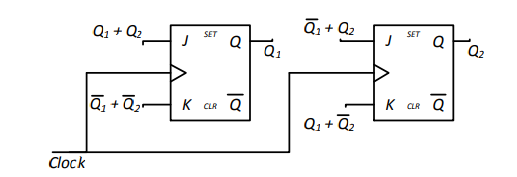
\includegraphics[width=\columnwidth]{question44.png}
        \caption{$2$-bit synchronous counter}
        \label{fig:enter-label}
    \end{figure}
    \begin{enumerate}
        \item $00\rightarrow11\rightarrow10\rightarrow01\rightarrow00...$ 
        \item $00\rightarrow01\rightarrow10\rightarrow11\rightarrow00...$
        \item $00\rightarrow01\rightarrow11\rightarrow10\rightarrow00...$
        \item $00\rightarrow10\rightarrow11\rightarrow01\rightarrow00...$
    \end{enumerate}
    \end{enumerate }
\section{\textbf{Components}}
\begin{tabularx}{0.46\textwidth}
    { 
      | >{\centering\arraybackslash}X 
      | >{\centering\arraybackslash}X 
      | >{\centering\arraybackslash}X
      | >{\centering\arraybackslash}X |
    }
    \hline
    \textbf{Component}& \textbf{Values} & \textbf{Quantity}\\
    \hline
    Arduino & UNO & 1 \\  
    \hline
    JumperWires & M-F & 25 \\ 
    \hline
    JK-Flip flop & 7476 & 1\\
    \hline
    OR Gate & 7432 & 1\\
    \hline
    Bread board & & 1\\
    \hline
\end{tabularx}
\section{\textbf{Connections}}
\begin{figure}[H]
    \centering
    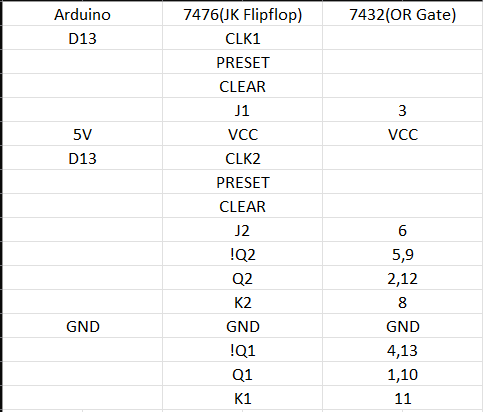
\includegraphics[width=0.8\columnwidth]{counter connections.png}
    \caption{Connections}
    \label{fig:enter-label}
\end{figure}

\section{\textbf{Procedure}}
\begin{enumerate}
    \item Connect the circuit as per the above table. 
    \item Connect the LED's to see the binary output sequence $0,1,3,2$
\end{enumerate}
\\ \begin{tabularx}{0.46\textwidth} { 
  | >{\centering\arraybackslash}X |}
  \hline
 https://github.com/Tangallamudi-RamaSai/Platformio/blob/main/platformio.ino.ino\\
  \hline
\end{tabularx}
\section{\textbf{Output}}
\begin{figure}[!ht]
    \centering
    \includegraphics[width=0.8\columnwidth]{counter.jpg}
    \caption{Output}
    \label{fig:enter-label}
\end{figure}
 \bibliographystyle{ieeetr}
\end{document}